% !TEX TS-program = pdflatex
% !TEX encoding = UTF-8 Unicode

% TO COMPILE: lmake (animal scrifices may be necessary)
%%%%%%%%%%%%%%%%%%%%%%%%%%%%%%%%%%%%%%%%%%%%%%%%%%%%%%%%%%%%%%%%%%%%%%%%%%
%																							                           %
%				                         PREAMBLE      							             %
%                                                                        %
%%%%%%%%%%%%%%%%%%%%%%%%%%%%%%%%%%%%%%%%%%%%%%%%%%%%%%%%%%%%%%%%%%%%%%%%%%
\documentclass[compress]{beamer}

\mode<presentation>
{
  \usetheme{Frankfurt}
  \usecolortheme{crane}
  \setbeamercovered{transparent}
}

% Package Setup
%%%%%%%%%%%%%%%%%%%%%%%%%%%%%%%%%%%%%%%%%%%%%%%%%%%%%%%%%%%%%%%%%%%%%%%%%%
%                                                                        %
%                                 PREAMBLE                               %
%                                                                        %
%%%%%%%%%%%%%%%%%%%%%%%%%%%%%%%%%%%%%%%%%%%%%%%%%%%%%%%%%%%%%%%%%%%%%%%%%%

%% PACKAGES
\usepackage[]{lineno}
\usepackage{fancyvrb}
%\linenumbers
\usepackage{amsmath}
\usepackage{microtype}
\usepackage{algorithmic}

%% GRAPHICS RELATED
\usepackage{graphicx}
\usepackage[outdir=./tmp/]{epstopdf}
\graphicspath{{../images/}{./}{./tmp/}}
\DeclareGraphicsExtensions{.eps, .pdf, .jpeg, .png}

%% CAPTION SETUP
\usepackage{float}
\usepackage[font=footnotesize]{caption}
\usepackage[font=small]{subcaption}
\captionsetup{belowskip=12pt,aboveskip=4pt}

%% BEAMER
\usepackage{multicol}
\usepackage{multirow}
\usepackage{array}				% Table Stuff
\usepackage{arydshln}
\usepackage{rotating}

%% BIBLIOGRAPHY
\bibliographystyle{ieeetr}

%% UNITS
\usepackage{siunitx}

%% EQUATIONS
%\numberwithin{equation}{section}

%%%%%%%%%%%%%%%%%%%%%%%%%%%%%%%%%%%%%%%%%%%%%%%%%%%%%%%%%%%%%%%%%%%%%%%%%%%
%                                                                         %
%                             Listing Setup                               %
%                                                                         %
%%%%%%%%%%%%%%%%%%%%%%%%%%%%%%%%%%%%%%%%%%%%%%%%%%%%%%%%%%%%%%%%%%%%%%%%%%%
\usepackage{listings}
\lstset{ %
    language=C++,
    basicstyle=\footnotesize\ttfamily,
    numbers=left,
    numberstyle=\tiny\color{gray},
    stepnumber=2,
    numbersep=5pt,
    backgroundcolor=\color{white},
    showspaces=false,
    showstringspaces=false,
    showtabs=false,
    frame=single,
    rulecolor=\color{black},
    tabsize=2,
    breaklines=true,
    breakatwhitespace=false,
    title=\lstname,
    keywordstyle=\color{blue},
    commentstyle=\color{OliveGreen},
    stringstyle=\color{orange}
}
\DeclareCaptionFont{white}{\color{white}}
\DeclareCaptionFormat{listing}{\colorbox[cmyk]{0.43, 0.35, 0.35, 0.01}{\parbox{\dimexpr\textwidth-2\fboxsep\relax}{#1#2#3}}}
\captionsetup[lstlisting]{format=listing,labelfont=white,textfont=white,singlelinecheck=false,margin=0pt,font={bf,footnotesize}}
%\lstnewenvironment{code}[1][]%
%{ \noindent\minipage{\linewidth}
%	\lstset{#1}
%}
%{\endminipage}
%% USER COMMANDS
\usepackage{isotope}
\newcommand{\iso}{\isotope}
\newcommand{\figurewidth}{\textwidth}
\newcommand{\micron}{$\mu$m}



% Preamble / Frst Size
%\setbeamersize{text margin left=5mm, text margin right 5mm}
\title[RPM8 Optimization] {Optimization of the RPM8 Detector with Genetic Algorithms}
\author[] {
    Matthew Urffer\inst{1}
}
\institute[University of Tennessee] { 
  \inst{1}%
  Department of Nuclear Engineering,
  University of Tennessee, Knoxville, TN
}

\date[] {March 3, 2013}
\pgfdeclareimage[height=0.5cm]{university-logo}{../images/utwordmarkhorz.png}
\logo{\pgfuseimage{university-logo}}

\begin{document}

\begin{frame}[plain]
  \titlepage
  \tiny
    \begin{center}
\centering{Financial support from the Domestic Nuclear Detection Office (DNDO) through Award No. 003387891 is gratefully acknowledged. 
  Any opinions, findings, and conclusions or recommendations expressed in this material are those of the presenter and do not necessarily reflect the views of DNDO.}
  \end{center}
\end{frame}

\begin{frame}{Table of Contents}
  \begin{multicols}{2}
    \tableofcontents
  \end{multicols}
\end{frame}


%%%%%%%%%%%%%%%%%%%%%%%%%%%%%%%%%%%%%%%%%%%%%%%%%%%%%%%%%%%%%%%%%%%%%%%%%%
%                                                                        %
%                          START OF CONTENT                              %
%                                                                        %
%%%%%%%%%%%%%%%%%%%%%%%%%%%%%%%%%%%%%%%%%%%%%%%%%%%%%%%%%%%%%%%%%%%%%%%%%%
\section{Introduction}
\subsection*{}
\begin{frame}{Introduction}
What geometry is best for the RPM8?
\begin{figure}
    \centering
    \begin{subfigure}[b]{0.25\textwidth}
        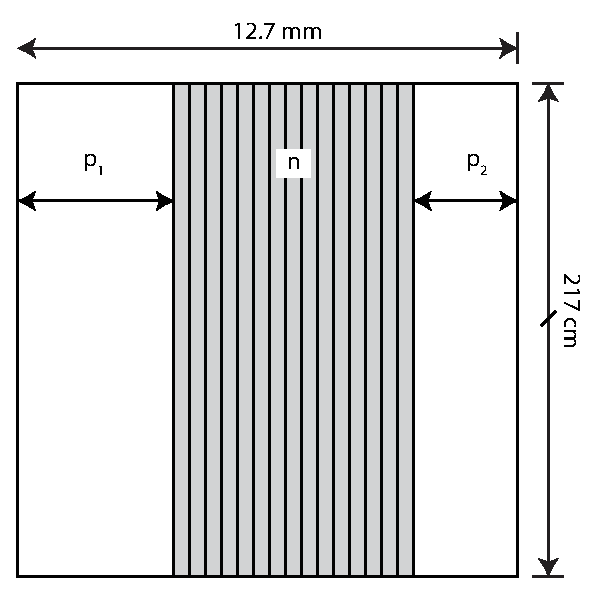
\includegraphics[width=\textwidth]{RPM8_Diagrams_OptDesign_A}
    \end{subfigure}
    ~
    \begin{subfigure}[b]{0.25\textwidth}
        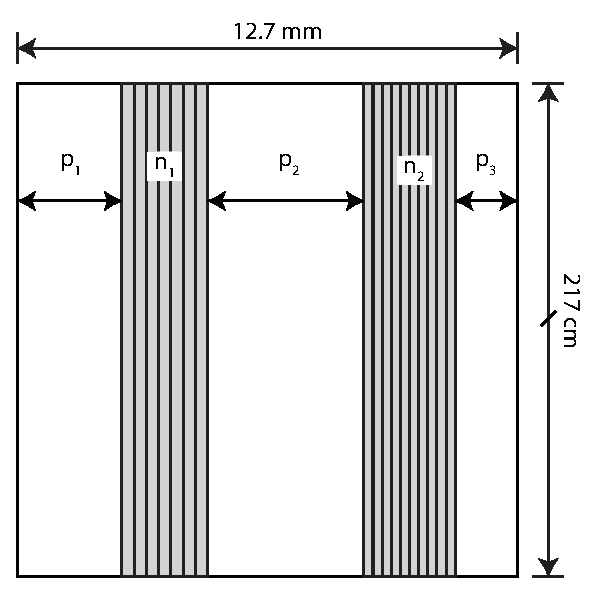
\includegraphics[width=\textwidth]{RPM8_Diagrams_OptDesign_B}
    \end{subfigure}

    \begin{subfigure}[b]{0.25\textwidth}
        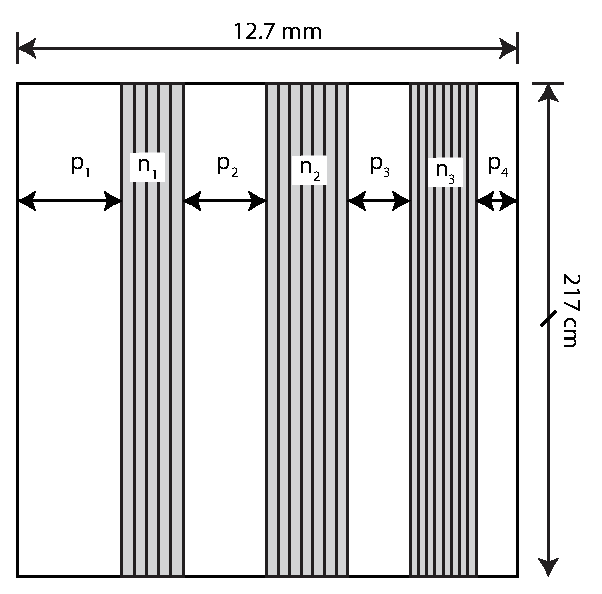
\includegraphics[width=\textwidth]{RPM8_Diagrams_OptDesign_C}
    \end{subfigure}
    ~
    \begin{subfigure}[b]{0.25\textwidth}
        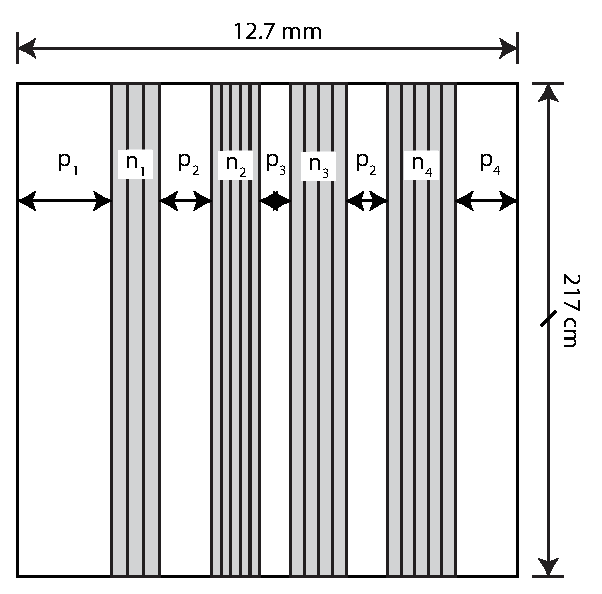
\includegraphics[width=\textwidth]{RPM8_Diagrams_OptDesign_D}
    \end{subfigure}
    \label{fig:OptDesignSchematics}
\end{figure}
Neturons will be moderated as they travel through the material, then wipped out by the absorber.
\end{frame}
%%%%%%%%%%%%%%%%%%%%%%%%%%%%%%%%%%%%%%%%%%%%%%%%%%%%%%%%%%%%%%%%%%%%%%%%%%
\begin{frame}{Design Constraints}
What do we mean by best?
\begin{itemize}
	\small
  \item Count rate? 
  \item Light output?
	\item Lowest cost / fabrication ease?
\end{itemize}
The design parameters were then:
\begin{itemize}
	\small
  \item The detector material
  \item The thickness of the detector material
  \item The spacing of detector layers
  \item The initial moderator thickness
\end{itemize}
\end{frame}
%%%%%%%%%%%%%%%%%%%%%%%%%%%%%%%%%%%%%%%%%%%%%%%%%%%%%%%%%%%%%%%%%%%%%%%%%%
\subsection{Previous Work}
\begin{frame}{Previous Work}
\begin{itemize}
	\small
	\item Have a working MCNPX model of the geometry
	\item Previous focused on a linear spacing of the films (simple)
	\item Have an idea on what thickness of moderator is necessary
		\begin{figure}
			\centering
			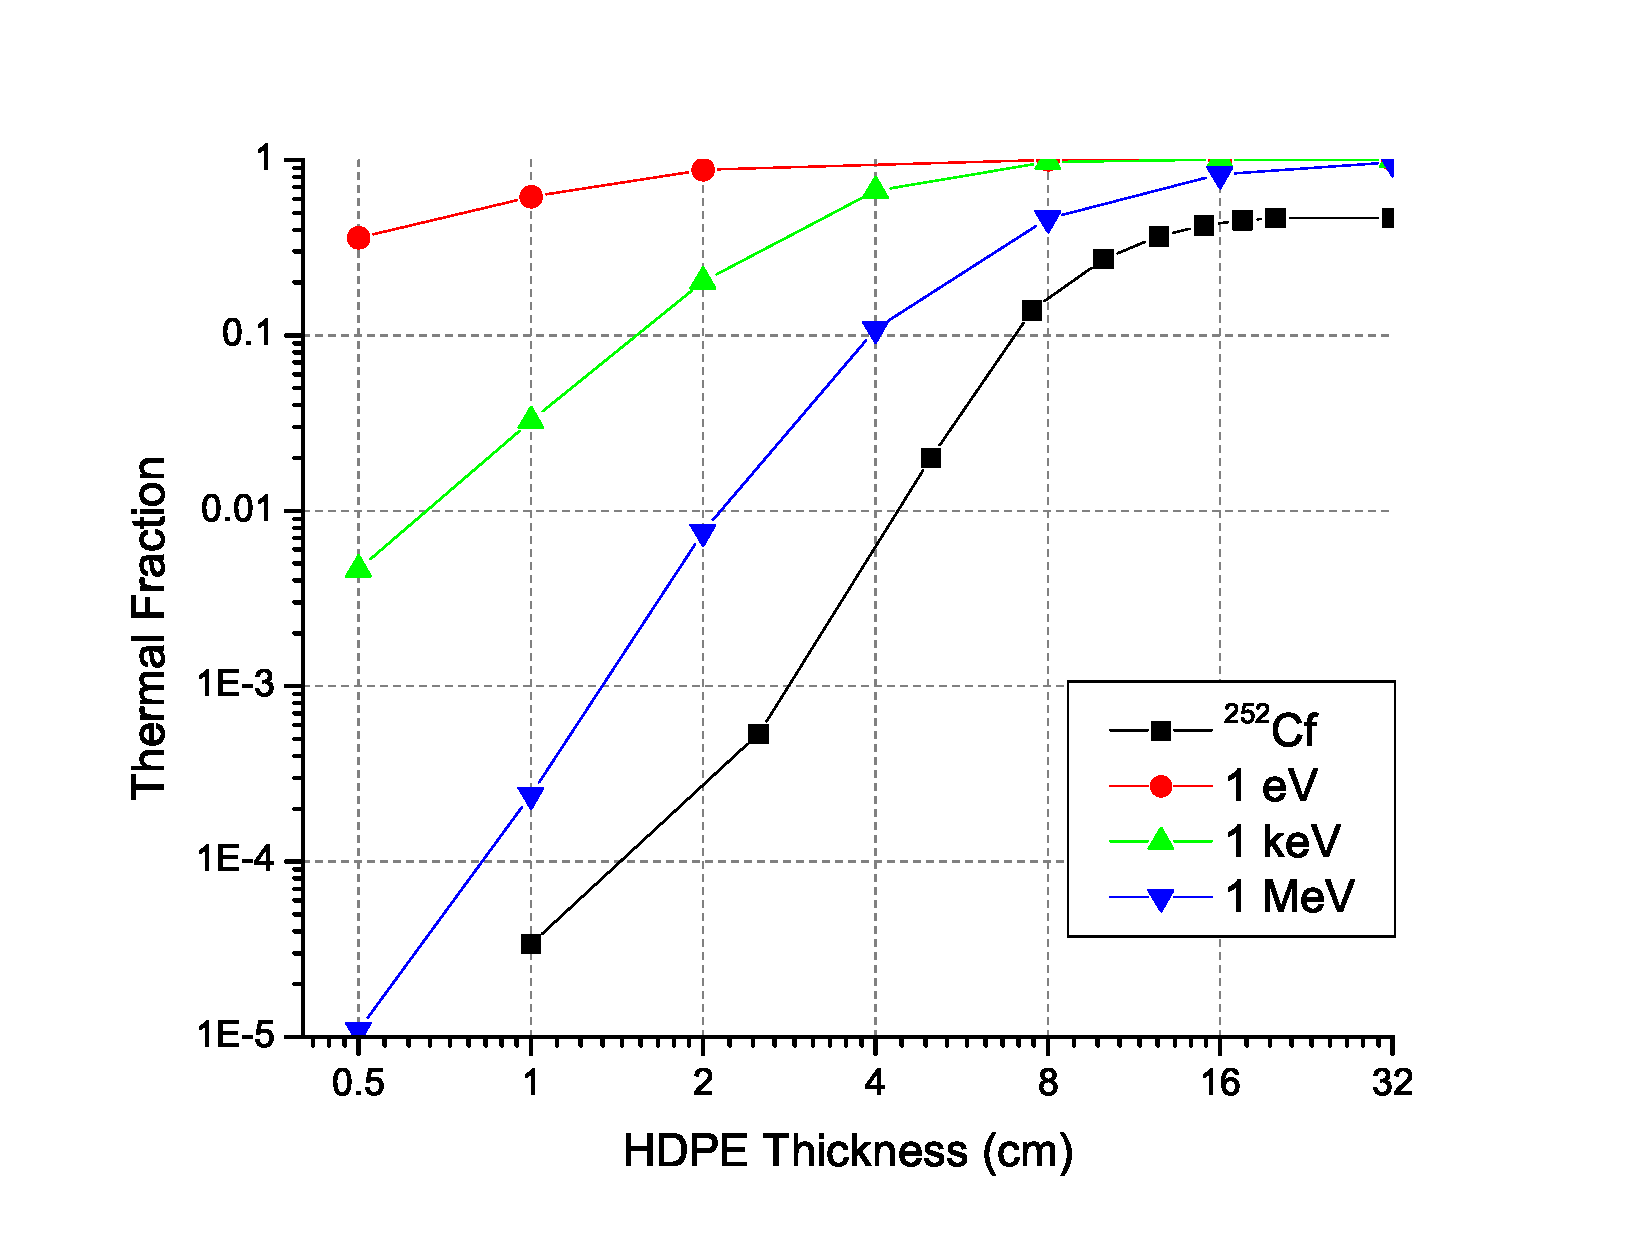
\includegraphics[width=0.75\textheight]{HDPEModThermalFraction}
		\end{figure}
	\item Don't know where the films go in the center
\end{itemize}
\centering
Optimization Problem!
\end{frame}
%%%%%%%%%%%%%%%%%%%%%%%%%%%%%%%%%%%%%%%%%%%%%%%%%%%%%%%%%%%%%%%%%%%%%%%%%%
\section{Genetic Algorithms}
%% Genatic Algorthims introduction

%%%%%%%%%%%%%%%%%%%%%%%%%%%%%%%%%%%%%%%%%%%%%%%%%%%%%%%%%%%%%%%%%%%%%%%%%%
\begin{frame}[fragile]{Choices, choices}
\centering
\tiny
\begin{Verbatim}[frame=single]
    ----------------------------------------------------------
                                                        F FN  
                                             F 5       F U  55
                                   F     F 5F  F     FFqBBMG05
                         F       FF1     N05 BBM F   F U8BBBMO
                      FF1       5 ZE     NN NBBB FF    1GMBB0 
                     F50Z5 F   1FMBBOF   F 5M20G  FF  5NBEOM 2
                    FFEBBB    5 M NM      5NBOO 8Bq   U8BBBBF5
                   1qZN MBZF F5OBME2F    F5Z8EB OZ   5 BBBBB 2
           5 F   F5MG M125   2BGMNF5     2MMM8MMF5   FBBBBBO 5
         UFF0 55  FEBMZGGF F  5BOGGN F   F5ZBNqB 5   1FBBZ GGG
    BNF5FGBN5BBNF FBBBBB 8E   5BMZO8q     2BBG 02     5BBB 1uq
    B 5q0BBBZqOq F1BBM5 51OZ 5 BB 5UE0     UBZN2     2ZBBBBEUU
    B OBBBBBG12 F 1BBO5 2F5   UEBBG2EBF   51BBBNU     JBBBBBG2
    BBBOG0BBB1 F  5 B qBB0 F 1uMB8B0FF   F2 BBBB F F U BB2 BBM
    B0MBB 0BB1F FFUUGBuNBM1 F ZB0j0OF   1 OBM 80    U8BBE5jNB8
    BUZBMZEFMNFF NMBBGFGB2  18BZ1UOB 5   OBq2UBEFF 1 BBq21 UBB
    BOG 5B 56BF 1BB0  UMB 5  BNUF FBM51 B8UFF5NBUF5FBB5UF 52MB
    BB 2 MZNZB 5 EqU 5 qM EFZGMq F5EBNZ  0 F 5 BMEZ BBB    2EB 
    ----------------------------------------------------------
    Symbolic Regression with Genetic Programing
    Matthew J. Urffer (matthew.urffer@gmail.com)
\end{Verbatim}
\end{frame}
%%%%%%%%%%%%%%%%%%%%%%%%%%%%%%%%%%%%%%%%%%%%%%%%%%%%%%%%%%%%%%%%%%%%%%%%%%
\subsection{PyEvolve}
%%%%%%%%%%%%%%%%%%%%%%%%%%%%%%%%%%%%%%%%%%%%%%%%%%%%%%%%%%%%%%%%%%%%%%%%%%
%                                                                        %
%                      Pyevole Introduction                              %
%                                                                        %
%%%%%%%%%%%%%%%%%%%%%%%%%%%%%%%%%%%%%%%%%%%%%%%%%%%%%%%%%%%%%%%%%%%%%%%%%%
\subsection{PyEvolve}
\begin{frame}{PyEvolve Introduction}
	\begin{itemize}
  \small
  \item PyEvolve is a genetic algorithm framework written in pure python
  \item Genetic Algorithm Features:
    \begin{itemize}
      \item Crossover operations (single point, two point, uniform)
      \item Mutator operations (swap, flip)
      \item Selection operations (rank, uniform, tournament, roulette)
    \end{itemize}
  \item Additional Features:
    \begin{itemize}
      \item Run statistics
      \item Convergence criteria
      \item Function callbacks
    \end{itemize}
  \end{itemize}
  \begin{figure}
    
\includegraphics[width=0.2\textwidth]{PyEvolveLogo.png}
  \end{figure}
\end{frame}
\begin{frame}{PyEvolve - Belly of the Lizard}
	Representation of the the Genetic Algorithm
  \begin{itemize}
    \item \texttt{GSimpleGA} genetic algorithm
    \item \texttt{GPopulation} - the population
    \item \texttt{Initializators} - initialization methods
    \item \texttt{Mutators} - collection of mutator methods
    \item \texttt{Crossovers} - collection of crossover methods
    \item \texttt{Selectors} - collection of selection methods
  \end{itemize}
  Representation of an individual
  \begin{itemize}
    \item Bit string representation \texttt{10010101}
    \item Defined in \texttt{G1DBinaryString.py}
		\item Other representations are available (tree, 2D list)
  \end{itemize}
\end{frame}

%%%%%%%%%%%%%%%%%%%%%%%%%%%%%%%%%%%%%%%%%%%%%%%%%%%%%%%%%%%%%%%%%%%%%%%%%%
\section{Methods}
\section{Methods}
\label{sec:Methodes}

The optimization of the films was formulated as finding the minimum mass of \iso[6]{Li} for a given detector material necessary to fulfill an interaction rate of \SI{2.5}{cps\per\nano\gram\iso[252]{Cf}} while maintaining a intrinsic gamma rejection ratio of \num{1.e-6}.

It is assumed that there is a fixed cost to assemble each detector assembly and mount it between the moderator.

\todo[inline]{Cost Trade-off section. In detector designs there can never be too much reflector based on a neutronics perspective, however at some point the moderator serves to reflect neutrons back to the source.}

\subsection{Design Parameters}
\label{sec:DesignParameters}
The design parameters were then:
\begin{itemize}
  \item The detector material. Materials with a high \iso{6}[Li] concentration will absorb more neutrons.
  \item The thickness of the detector material.
  \item The spacing of detector layers.
  \item The initial moderator thickness.
\end{itemize}

The geometry is described as follows:
There is an initial moderator of \SI{2.5}{\centi \meter} HDPE to achieve a thermal fraction around 10\%.
\footnote{The thermal energy was chosen to be \SI{5}{\electronvolt}. 
The \isotope[6]{Li} neutron cross section as this energy is 67 barns. 
A sample containing 10\% \iso[6]{Li} and a density of\SI{1.0}{\gram \per \cubic \centi\meter} would then macroscopic cross section of \SI{0.67}{\per \centi\meter}, attenuating \SI{0.67}{\percent} of the incident flux in \SI{0.01}{ \centi\meter}. 
The macroscopic cross section calculation is shown below. 
\begin{align*}
\Sigma &= \frac{\rho N_A}{M}  \left ( n_1 \sigma_1 + n_2 \sigma_2 + n_3 \sigma_3 + \dots  \right ) \\ 
       &= \frac{\rho N_A n_1 \sigma_1}{M} \\
       &= \frac{\SI{1.0}{\gram\per\cubic\centi\meter} \SI{6.022E23}{\per\mole} \SI{67}{\barn}{0.05}}{6} \\
       &= \SI{0.67}{\per\centi\meter} 
\end{align*}
}..
Following the moderator there are repeated sections of detector assembly and moderator.
A single detector assembly consists of a layered film \SI{100}{\micron} thick with a light guide of \SI{0.5}{\centi\meter}.
After the absorb film and light guide assemblies is additional moderator.
Four basic detector designs were considered, as shown in Figure ~\ref{fig:OptDesignSchematics}
In the first design there are only three parameters; the thickness of the moderator $P_1$, the thickness of the reflector $P_2$ and the number of layers, $n$. 
In the second detector design (B) there are two assemblies of layered detectors surrounded by HDPE moderator.  Thus there are five parameters to optimize; the thickness of the front moderator $p_1$, the thickness of the moderator separating the assemblies $p_2$, the thickness of the reflector $p_3$, and the number of films in each assembly, $n_1$ and $n_2$.
Similarly there are seven parameters to optimize in design C, and nine parameters to optimize in design D.

\begin{figure}
    \centering
    \begin{subfigure}[b]{0.45\textwidth}
        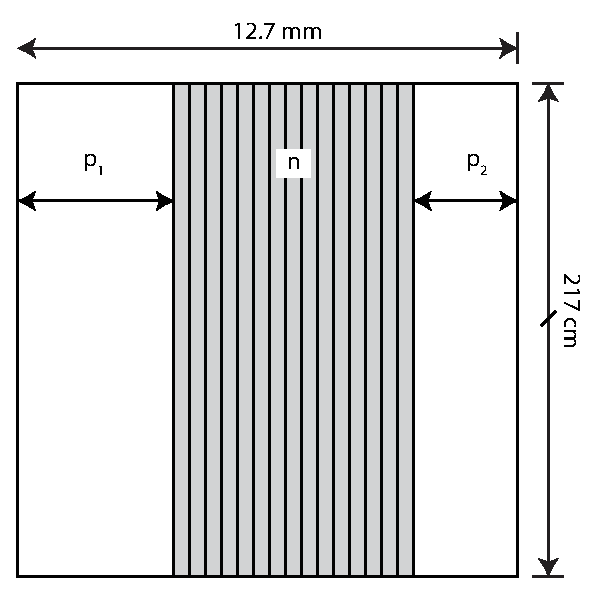
\includegraphics[width=\textwidth]{RPM8_Diagrams_OptDesign_A}
        \caption{A single detector assembly}
    \end{subfigure}
    ~
    \begin{subfigure}[b]{0.45\textwidth}
        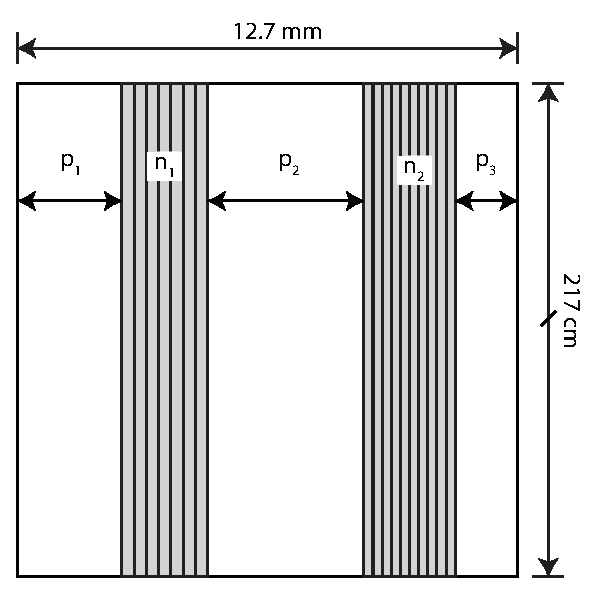
\includegraphics[width=\textwidth]{RPM8_Diagrams_OptDesign_B}
        \caption{Two detector assemblies}
    \end{subfigure}

    \begin{subfigure}[b]{0.45\textwidth}
        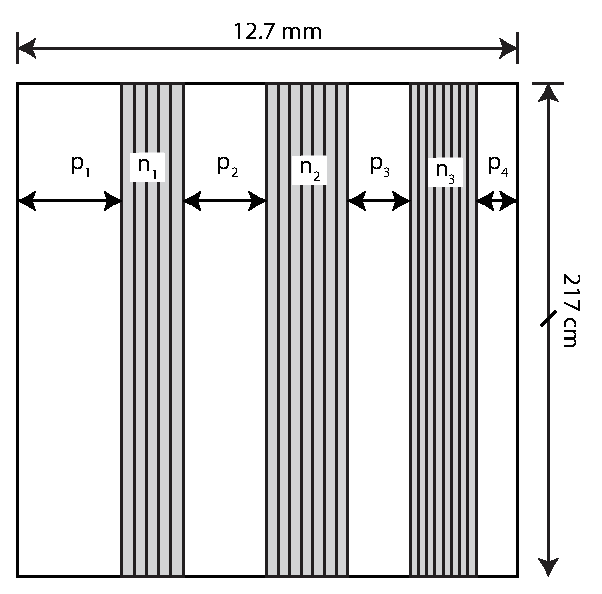
\includegraphics[width=\textwidth]{RPM8_Diagrams_OptDesign_C}
        \caption{Three detector assemblies}
    \end{subfigure}
    ~
    \begin{subfigure}[b]{0.45\textwidth}
        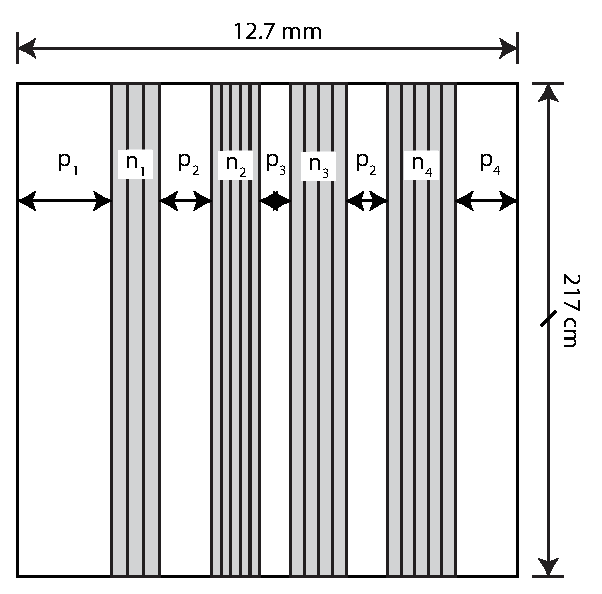
\includegraphics[width=\textwidth]{RPM8_Diagrams_OptDesign_D}
        \caption{Four detector assemblies}
    \end{subfigure}
    \caption{Detector Designs for Optimization}
    \label{fig:OptDesignSchematics}
\end{figure}

Figure ~\ref{fig:MCNPXRendering} shows the MCNPX renderings of the X-Z profile of two detector configurations.
The source is not shown as it is located \SI{2}{\meter} from the detector midpoint.

\begin{figure}
    \centering
    \begin{subfigure}[b]{0.45\textwidth}
        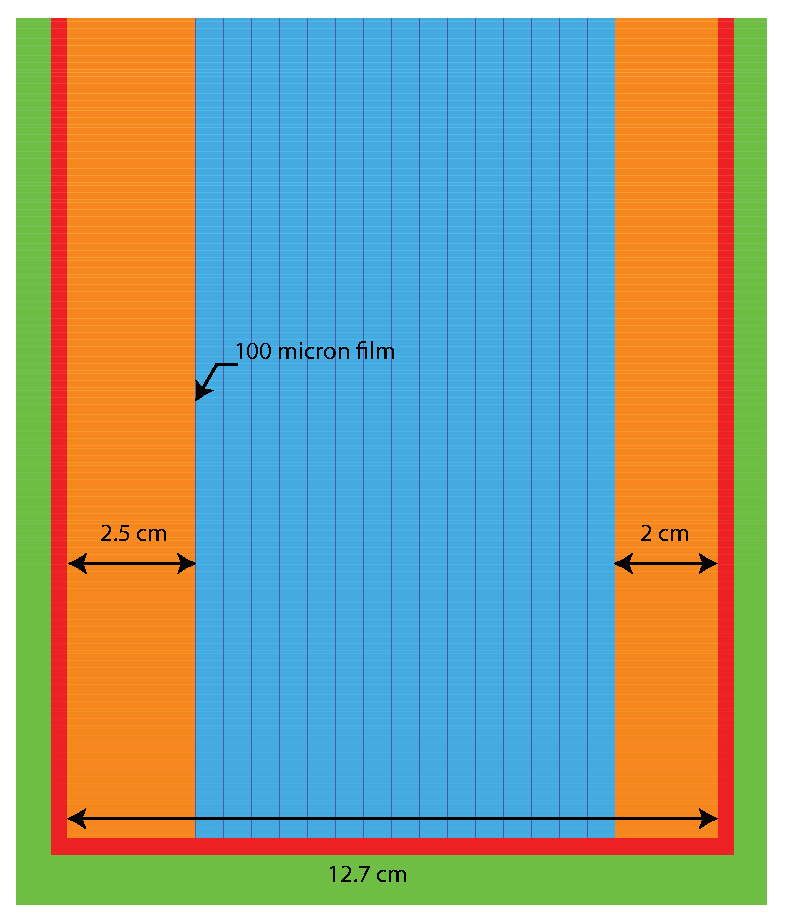
\includegraphics[width=\textwidth]{RPM8_Diagrams_MCNPXRender_1Assm}
        \caption{MCNPX Model of One Assembly}
    \end{subfigure}%
    ~
    \begin{subfigure}[b]{0.45\textwidth}
        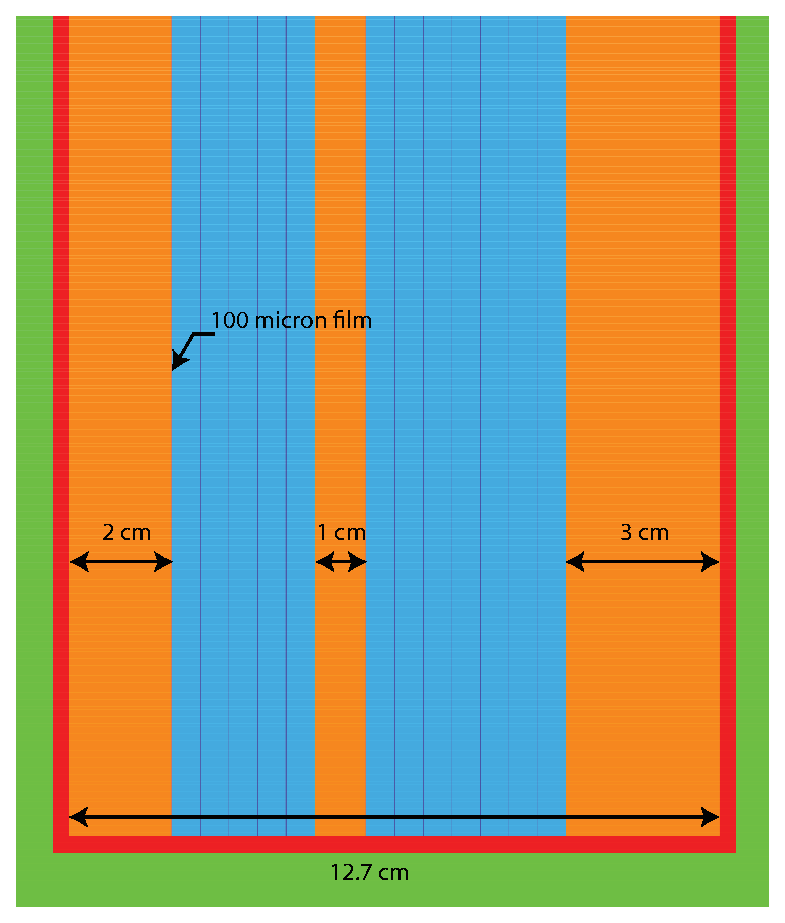
\includegraphics[width=\textwidth]{RPM8_Diagrams_MCNPXRender_2Assm}
        \caption{MCNPX Model of Two Assemblies}
    \end{subfigure}
    \caption{MCNPX rendering of layered geometry}
    \label{fig:MCNPXRendering}
\end{figure}
The optimization of the detector design is presented in two parts: a numerical approach in which a matrix of detector spacing and assemblies are varied (Section ~\ref{sec:MCNPXMethods}, and a multivariate-variate optimization in which the parameters are fit to a functional form which is then optimized (Section ~\ref{sec:MVOptimization}).
\subsection{MCNPX Simulations}
\label{sec:MCNPXMethods}
A matrix of detector designs was simulated in MCNPX, with the parameters are described in Table \ref{tab:MCNPXGeoMatrix}.
A generic script file was written (Listing ~\ref{lst:MCNPScript}) that was modified with the code in Listing ~\ref{lst:CreateSurfaceCell} to include a user supplied number of detector assemblies, spacing between these assemblies, and initial moderator at the front of the assembly.
The MCNPX output was post processed with the python modules presented in Listing ~\ref{lst:ParseOutput} and Listing ~\ref{lst:mctal}.
See ~\ref{sec:RPM8Listings} for detailed information on the developed scripts and details on the running of the problems.
\begin{table}
	\caption{Number of Film Assemblies and Spacing of MCNPX Simulations}
	\label{tab:MCNPXGeoMatrix}
  \centering
	\input{MCNPXGeoMatrix.dat}
\end{table}

Two tallies were used in the MCNPX calculations: the interaction rate tally (tally type 4) and the surface flux tally (type 2).
If the scalar flux is defined as $\phi(\vec{r},E,t)=\int d\Omega \Phi(\vec{r},\hat{\Omega},E,t)$ the  interaction rate tally is the integral of all energies and directions of the scalar flux over a given volume, normalized by that volume ~\eqref{eqn:F4TallyDef}.
This quantity is then modified by an FM card which calculates quantities of the form $Q = C \int {\Phi(E) R_m(E) dE }$ where:
\begin{itemize}
    \item $C$ is a scalar normalization (density)
    \item $R_m(E)$ is the response function
    \item $\Phi(E)$ is the neutron flux
\end{itemize}
Similarly the surface flux is the integral over the entire surface (normalized by the surface area) of the scalar flux, as shown in \eqref{eqn:F2TallyDef}.
\begin{align}
    \label{eqn:F4TallyDef}
    \bar{\phi_V} = \frac{1}{V}\int dE \int dt \int dV \int d\Omega \AngularFlux
\end{align}
\begin{align}
    \label{eqn:F2TallyDef}
    \bar{\phi_S} = \frac{1}{A}\int dE \int dt \int dA \int d\Omega \AngularFlux
\end{align}
\todo[inline]{The F2 tally currently is not being used, only the F4 tally interactions}
The FM card can modify any flux or current tally of the form $\int \psi (E) dE$ into $\int R(E)\psi(E) dE$, where $R(E)$ is the response function known to MCNP.
\subsection{1 D Transport Part}
The large detector and far away source suggest that the problem can be simplified into a one dimensional transport problem without suffering the accuracy of the solution.
As 1D deterministic transport is much faster than 3D Monte Carlo, 1D transport was explored in order to vary the problem parameters.

A matrix of \SI{25}{\percent} \iso[6]{Li} PEN films were completed with the film assemblies being 1,2,3, and 4 and with a spacing of \SI{1}{\centi\meter},\SI{2}{\centi\meter},\SI{3}{\centi\meter},and \SI{4}{\centi\meter}. 


\subsection{Multivariate Optimization}
\label{sec:MVOptimization}

The multivariate optimization problem was formulated as finding $\min_{\vec{x}} f (\vec{x})$ subject to constraints, where $f(\vec{x})$ is the response function.

\subsubsection{Genetic Algorithm}
\label{sec:GeneticAlgoMethods}
Genetic algorthims provide a search method analous to biological evoluation.
Rather than following a gradient of a response function, genetic algorthims generate possible hypothesis by repeatably applying genetic operators (mutation and recombination) of the best currently known hypothesis in order to generate new ones\todo{CIte Mitchel}.
In this way the search space of canidate hypothesis (possible detector designs) is searched to identify the best hypothesis; the design that uses the least amount of \iso[6]{Li} while meeting the critera.
The genetic algorithm typically consist of four tasks: creating an initial population, evaluating that populations fitness, selecting members of the current population to breed, and then applying genetic operators to the selected members to breed the new population. 
This is completed for either a maximum generation is reached or the desired fitness is achieved. 

\begin{figure}
\begin{algorithmic}
  \WHILE{$error>goal$}
		\FORALL{$p \in P$}
			\STATE{Compute fitness}
		\ENDFOR
		\FORALL{$p \in P$}	
			\STATE{Choose individuals based on fitness}
			\STATE{Select individuals for next population}
			\STATE{Crossover selected individuals}
			\STATE{Mutate selected individual}
		\ENDFOR
	\ENDWHILE
\end{algorithmic}
\caption{Genetic Program Outline}
\label{AlgoOutline}
\end{figure}

The genome representation of the geometry was chosen to be represented as a bit string of a set length.
Each \verb+1+ or \verb+0+ in the string would represent a detector slice or a moderator slice, respectively.
For example the sequence \verb+0001110010+ would represent a detector that had three moderator slices, three detector slices, another two moderator slices, and a final detector slice before a single moderator slice as the reflector.
It was originally thought to have all of the moderator and detector slice the same thickness, \SI{0.5}{\centi \meter}\footnote{Astute readers may note that with a \SI{0.5}{\centi \meter} light guide and \SI{100}{\micro \meter} detector that the detector size is not \SI{0.5}{\centi\meter} and that 25 slices of \SI{0.5}{\centi\meter} each is \SI{0.2}{\centi\meter} short of the RPM8 size. However, it is not envisioned that \SI{20}{\milli\meter} will greatly impact the solution, or be within the manufacturing tolerances. }.
However, that would create 25 slices with a search space of $2^{25}$ or 33.5 million options.

\todo[inline]{A possibility would be to do a 2 centimeter reflector and a 2 centimeter reflector as constant.  This would then only have $2^{15}$ options, 32,000. I don't want to mess with different sized layers, because then my genomes are different lengths, and it becomes difficult to ensure that it is a correct geometry}.

The fitness function was choosen to count rate per mass of \iso[6]{Li}, provided that the geometry meet the total count rate criteria.
If it failed to meet the count rate criteria a zero fitness was returned \eqref{eqn:FitnessFun}.
\begin{align}
    \label{eqn:FitnessFun}
    f(\vec{x})
    = \begin{cases}
    0 & \text{if} \text{countRate}(\vec{x}) \leq \SI{2.5}{cps\per\nano\gram\iso[252]{Cf}} \\
    \text{countRatePerMass}(\vec{x})
    \end{cases}
\end{align}
\todo[inline]{Implmeneation of the fitness function might be completed by a dictionary of precomputed geometries. Interlopation could then be used to calculate the interaction of new geometries, and these could then be added to the dictionary.  An ANN might be used for the interoplation, and then retrained (or maybe online training) after a certain number of new hypothesis are made.  It might be useful to have some sort of degree of similarity between hypothsis. One might be logical and of the two hypothesis. In this case 0 would be the same, and len(hypothesis) would be the most disimilar.  Maybe if they are greater than 25 percent different we would want to run the case and add it?}

The mutation operation was chosen to be a simple bit flip in which a randomly chosen \verb+1+ or \verb+0+ in the geoemtry was flipped; for example \verb+001001010+ could be mutated to \verb+001001000+.
Crossover, in which two individuals are breed in produce the new generataion was implemented as \textbf{VALUE}.
\todo[inline]{I need to find out what crossover is used, either two-point, one-point, or uniform.}
An example of the crossover operations is shown in the Figure ~\ref{figGeneticCrossover}.
\begin{figure}
    \missingfigure{Crossover examples}
    \caption[Genetic Crossover Operations]{Genetic Crossover Operations}
    \label{fig:GeneticCrossover}
\end{figure}

The pyevolve toolkit was used for running of the genetic algorthim.
The genetic algorthim used a mutation rate of 2\%\todo{Check Mutation Rate} and a crossover rate of 80\%\todo{Check crossover rate}.
Tournamnet selectrion was used to determine which individuals would be allowed to breed for the next generation.
\todo[inline]{There is also the possibility to bootstrap to be population by variations on the best from previous generations.}
The accuracy of the genetic algorthim was checked by hand in simplified geometries.
As shown in Table \ref{tab:BitStringGeo} some of the these geometries are simple enougth that the search space can be computed exaustively.
\begin{table}
    \caption[Genome Bit String Geometries]{Bit String Simplified Geometetry Descriptions}
    \label{tab:BitStringGeo}
    \centering
    \begin{tabular}{ c | c c c c}
        Genome Length&Films Per Assembly&Slice Thickness&Light Guide Thickness&Possible Geomeries \\
        \hline
        \hline
        3&4&4.23&1.058&7 \\
        4&4&3.18&0.794&15 \\
        5&3&2.54&0.847&31 \\
        6&3&2.12&0.706&63 \\
        7&3&1.81&0.605&127 \\ 
        \hline
        10&3&1.27&0.423&1023 \\
        \hline
        13&2&0.98&0.488&8191 \\
        26&1&0.49&0.488&67108863 \\
    \end{tabular}
\end{table}
\todo[inline]{Could also do a little study about how we can then estimate the compute time needed for higher search spaces}



\section{Results}
\subsection{Validation}
\begin{frame}{Validation}
Validation of optimal solution can be observed directly for low dimensional searches
\begin{table}
    \caption[3 Bit Genome Results]{Bit String Simplified Geometry Descriptions}
    \label{tab:BitStringGeo}
    \centering
    \tiny
    \begin{tabular}{ p{1.5cm} | p{1.5cm} p{1.5cm}  p{1.5cm}}
			Genome&Mass Li-6&Count Rate& Count Rate per Mass \\
      \hline
      \hline
			010&16.7&2.9&0.175 \\ 
			\hline
			011&33.5&3.3&0.100 \\
			001&16.7&1.28&0.074 \\
			111&50.3&4.6&0.091 \\
			110&33.5&4.2&0.125 \\ 
			100&16.7&2.5&0.147 \\
			101&33.5&3.9&0.116 \\
      \hline
    \end{tabular}
\end{table}
Similarly for other low dimensional search spaces
\end{frame}

\begin{frame}[fragile]{Bootstrapped Genomes and Engineering Judgment}
\begin{itemize}
	\item Observed that all optimal solutions in low dimensions have moderator and reflector
	\item Possibility to reduce search space by setting moderator and reflector bits
	\item Possibility to initialize solutions for higher dimensions from lower ones
	\begin{itemize}
		\item Example: \verb+010+ $\to$ \verb+01000+ $\to$ \verb+0010000100000+
		\item Danger is not having enough diversity to avoid local minima
	\end{itemize}
\end{itemize}
\end{frame}

\begin{frame}[fragile]{Optimal Geometries}
\begin{table}
    %\caption[Optimal Bit String Geometries]{Genatic Algothrim Optimal Geometries}
    \centering
    \tiny
    \begin{tabular}{ p{0.75cm} | p{1cm} p{3.25cm} p{0.75cm} p{1cm} p{1cm}}
      Genome Length&Films Per Assembly&Optimal Geometry&Mass \iso[6]{Li}(g)&CPS per ng \iso[252]{Cf} & Count Rate per Mass \iso[6]{Li} (cps/g) \\
      \hline
      \hline
      3&4&\verb+010+&16.75&2.93&0.175 \\
      4&4&\verb+0100+& & & \\
      5&3&\verb+01000+&12.56&2.89&0.230 \\
      6&3&\verb+010000+&12.56&2.88&0.230 \\
      7&3&\verb+0100000+&12.56&2.84&0.226 \\ 
      10&3&\verb+0100000000+&12.56&2.68&0.214 \\
      10&3&\verb+0010000000+&12.56&2.93&0.233 \\
      10&3&\verb+0001000000+&12.56&2.95&0.235 \\
      13&2&\verb+00010010000000+&16.75&3.88&0.232 \\
      13&2&\verb+00100010000000+&16.75&3.90&0.233 \\
      13&2&\verb+00100100000000+&16.75&3.87&0.231 \\
      26&1&\verb+00000110110000000010000000+&20.94&4.33&0.206 \\
      26&1&\verb+00001010001000100000000000+&16.75&4.20&0.251 \\
    \end{tabular}
\end{table}
\end{frame}
%%%%%%%%%%%%%%%%%%%%%%%%%%%%%%%%%%%%%%%%%%%%%%%%%%%%%%%%%%%%%%%%%%%%%%%%%%
\begin{frame}{Optimal Geometries Rendered}
\begin{figure}
    \centering
    \begin{subfigure}[b]{0.45\textwidth}
        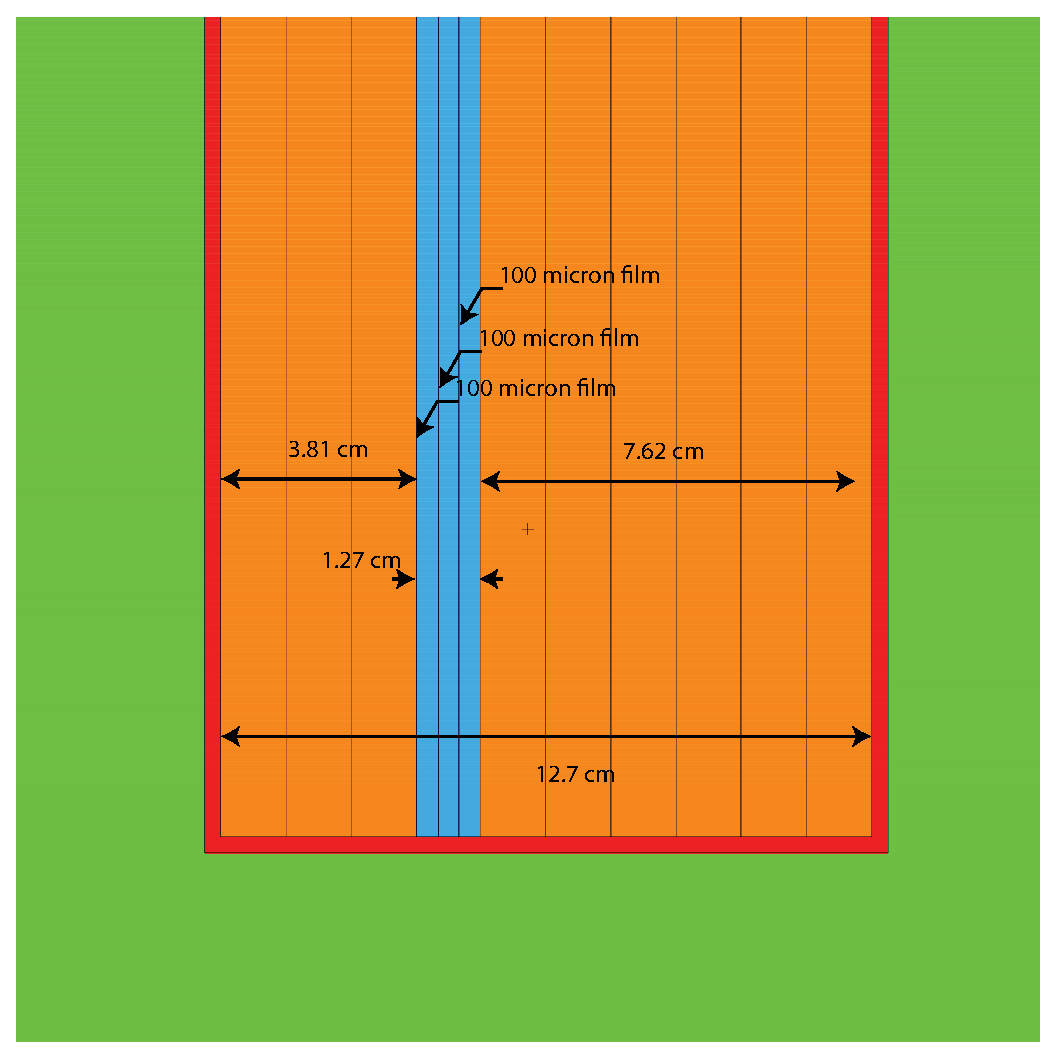
\includegraphics[width=\textwidth]{RPM8_Diagrams_MCNPXRender_10Opt}
    \end{subfigure}%
    ~
    \begin{subfigure}[b]{0.45\textwidth}
        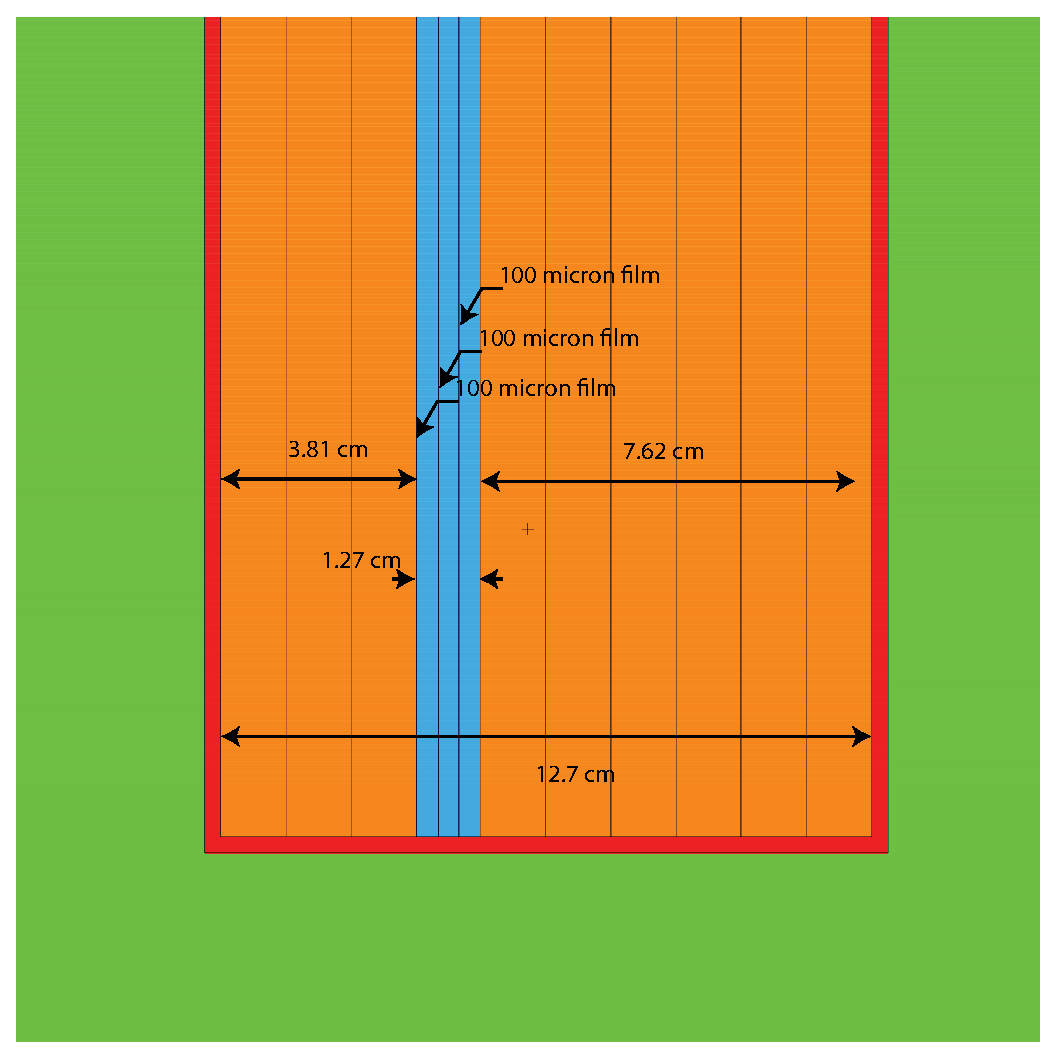
\includegraphics[width=\textwidth]{RPM8_Diagrams_MCNPXRender_26Opt}
    \end{subfigure}
    \caption{MCNPX rendering of layered geometry}
    \label{fig:MCNPXRendering}
\end{figure}
\end{frame}
%%%%%%%%%%%%%%%%%%%%%%%%%%%%%%%%%%%%%%%%%%%%%%%%%%%%%%%%%%%%%%%%%%%%%%%%%%
\subsection{Timing and Run Information}
\begin{frame}{Number of Geometries and Search Space}
Benefit of GA becomes apparent at higher search spaces!
\begin{table}
    %\caption[Optimal Bit String Geometries]{Genatic Algothrim Optimal Geometries}
    \centering
    \tiny
    \begin{tabular}{ p{0.75cm} | p{1cm} p{1cm} p{1cm} p{1cm} p{1cm}}
      Genome Length&Population Size&Number Runs&Average Generations&Fraction of Search Space Covered&Average Geometries Simulated \\
      \hline
      \hline
      3&6&20&4.6&100\%&24.5 \\
			4&8&18&3.8&100\%&30.7 \\
			5&10&18&6.0&100\%& 60.0 \\
			6&12&19&7.6&100\%&91.6 \\
			7&14&16&8.8&0.87\%&122.7 \\
			10&20&12&26.8&0.47\%& 536.7 \\
			13&26&8&19.0&0.18\% &494.0\\
			26&52&2&8.5&0.0014\% &442.0\\
    \end{tabular}
\end{table}
\end{frame}

\section{Conclusions}
%%%%%%%%%%%%%%%%%%%%%%%%%%%%%%%%%%%%%%%%%%%%%%%%%%%%%%%%%%%%%%%%%%%%%%%%%%
\begin{frame}{Summary}
Cost trade offs
\begin{itemize}
	\item Assumed \iso[6]{Li} was the most expensive part
	\item Fabrication cost for a complicated design might hinder this
	\item Is the space thick enough to get the light out?
\end{itemize}
Can significantly reduce the amount of \iso[6]{Li} needed
\end{frame}
\begin{frame}{Future Work}
\begin{itemize}
	\item Improve performance on GA
	\small
	\begin{itemize}
		\item Can play with mutation rate and crossover rate
		\item Can play with population size and selection
		\item Use PyEvolve multiprocessing instead of mine - might remove code sensitivity
	\end{itemize}
	\normalsize
	\item Use a 1D transport code
	\item Run for different materials
	\item More runs at higher lengths
\end{itemize}
\end{frame}
\begin{frame}
	\centering
\begin{figure}
  
\includegraphics[height=6cm]{Questions.eps}
\end{figure}
\end{frame}
%%%%%%%%%%%%%%%%%%%%%%%%%%%%%%%%%%%%%%%%%%%%%%%%%%%%%%%%%%%%%%%%%%%%%%%%%%%
% BILBIOLGRAPHY
%\begin{frame}[plain,allowframebreaks]
%\frametitle{Works Cited}
%	\tiny
%  \bibliography{../Zotero}
%\end{frame}

%%%%%%%%%%%%%%%%%%%%%%%%%%%%%%%%%%%%%%%%%%%%%%%%%%%%%%%%%%%%%%%%%%%%%%%%%%%
% APPENDIX
%%%%%%%%%%%%%%%%%%%%%%%%%%%%%%%%%%%%%%%%%%%%%%%%%%%%%%%%%%%%%%%%%%%%%%%%%%%
\begin{frame}{Geometry for HDPE Moderation}
\begin{figure}
  \begin{subfigure}[b]{0.45\textwidth}
    \centering
    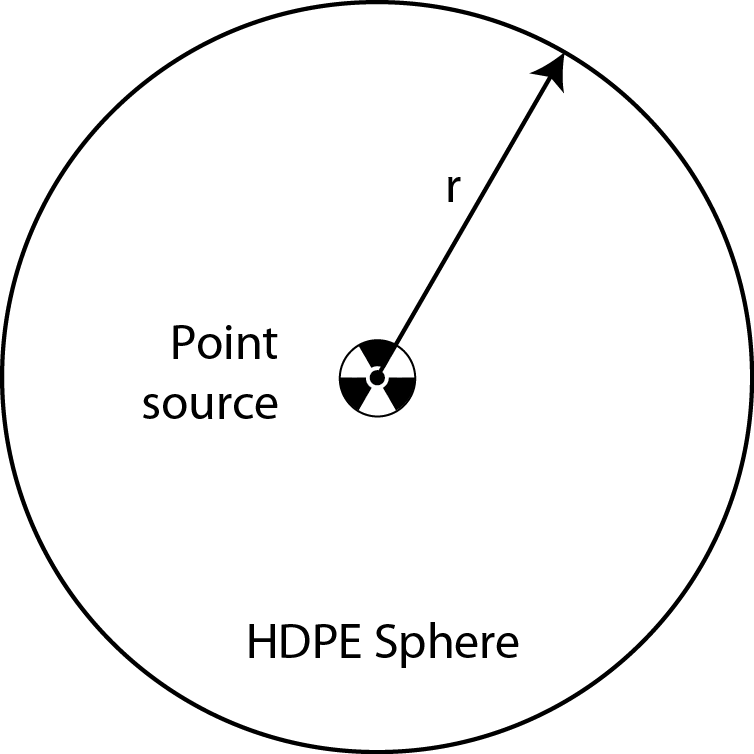
\includegraphics[width=\textwidth]{HDPEModeration_PointSrcGeo}
    \caption{Geometry of mono energetic point source}
  \end{subfigure}%
  ~
  \begin{subfigure}[b]{0.45\textwidth}
    \centering
    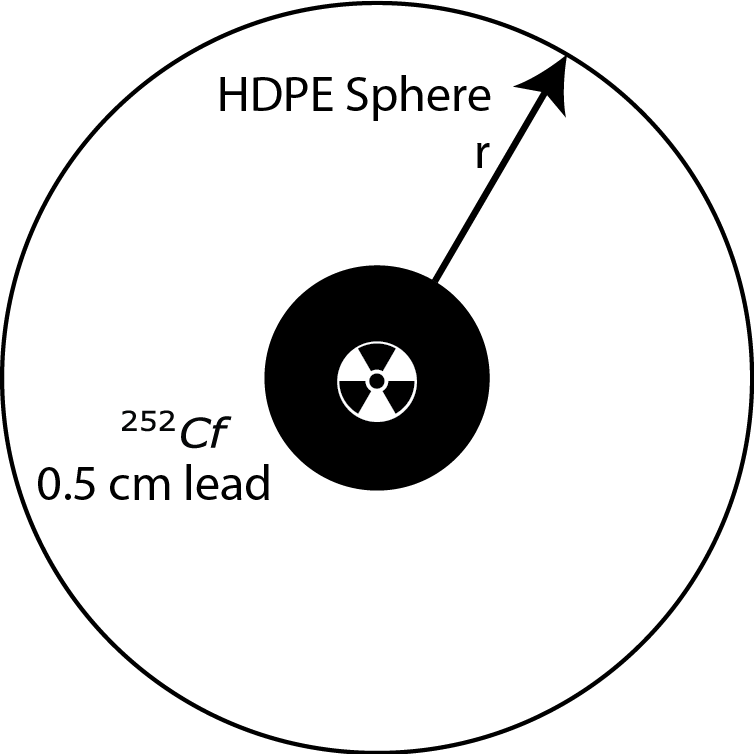
\includegraphics[width=\textwidth]{HDPEModeration_Cf252SrcGeo}
    \caption{Geometry of \isotope[252]{Cf} source}
  \end{subfigure}
  \caption{Simulated Geometry}
\end{figure}
\end{frame}
%%%%%%%%%%%%%%%%%%%%%%%%%%%%%%%%%%%%%%%%%%%%%%%%%%%%%%%%%%%%%%%%%%%%%%%%%%%

\end{document}


